\documentclass[10pt,aspectratio=169]{beamer}

% All the boilerplate is in deslides.sty
\usepackage{deslides}

\author{Ji\v{r}\'i Lebl}

\institute[OSU]{%
Oklahoma State University%
%Departemento pri Matematiko de Oklahoma {\^S}tata Universitato%
}

\title{17. Mechanical vibrations, part 1: free undamped motion\\(Notes on Diffy Qs, 2.4)}

\date{}

\begin{document}

\begin{frame}
\titlepage

%\bigskip

\begin{center}
The textbook: \url{https://www.jirka.org/diffyqs/}
\end{center}
\end{frame}

\begin{frame}
\textbf{Mass on a spring:}

\vspace*{-12pt}
\hspace*{3in}%
\scalebox{0.9}{\subimport*{../figures}{massfigforce.pdf_t}}

\vspace*{-0.55in}
$t = {}$ time in seconds.\\
$x(t) = {}$ displacement from rest, in meters.\\
$m = {}$ mass in kilograms.\\
$k = {}$ spring constant in newtons per meter.\\
$c = {}$ damping (friction) in newton-seconds per meter.\\
$F(t) = {}$ external force on the mass in newtons.

\medskip
\pause

Hooke's law: 
Force exerted by the spring is proportional to
compression spring: $-kx$.

\pause
Force exerted by damping is proportional to the velocity of mass: $-cx'$.

\pause
Newton's second law: Force equals mass times acceleration:
\[
mx'' = F(t)-cx'-kx
\pause
\qquad
\text{or}
\qquad
mx'' + cx' + kx = F(t) .
\]
\pause
Second order, linear, constant coefficient ODE.

\medskip
\pause

Motion is:

\vspace*{-12pt}%
\hspace*{1in}%
\emph{forced} if $F \not\equiv 0$, \quad and
\emph{unforced} or \emph{free} if $F \equiv 0$

\pause
\hspace*{1in}%
\emph{damped} if $c > 0$, \quad
and \emph{undamped} if $c = 0$.
\end{frame}

\begin{frame}
\textbf{RLC circuit:}

\vspace*{-12pt}
\hspace*{3in}%
\scalebox{0.9}{\subimport*{../figures}{mv-rlc.pdf_t}}

\vspace*{-0.45in}

Resistor: $R$ ohms.\\
Inductor: $L$ henries.\\
Capacitor: $C$ farads.\\
Electrical source: $E(t)$ volts.\\
$Q(t) = {}$ charge on the capacitor in coulombs.\\
$I(t) = {}$ current in the circuit in amperes.

\medskip
\pause

The basic relationships: $Q' = I$ and $L I' + RI + \nicefrac{Q}{C} = E$.

\medskip
\pause

Differentiate to get
\[
L I''(t) + R I'(t) + \frac{1}{C} I(t) = E'(t) .
\]
\end{frame}

\begin{frame}
\textbf{Linearized pendulum:}

\vspace*{-12pt}
\hspace*{3.2in}%
\scalebox{0.9}{\subimport*{../figures}{mv-pend-deriv.pdf_t}}

\vspace*{-1.4in}

$m = {}$ mass.

$\theta(t) = {}$ angle the pendulum makes with vertical.

$L = {}$ length of the pendulum (meters).

$g = {}$ force of gravity.

\medskip
\pause

Via Newton's second: force $-mg \sin \theta$ equals

mass $m$ times acceleration
$L \theta''$:

\medskip

\qquad
$
\displaystyle
mL\theta'' = -mg \sin \theta
\pause
\qquad
\text{or}
\qquad
\theta'' + \frac{g}{L} \sin \theta = 0 .
$

\pause

Nonlinear!

\medskip
\pause

But!  For $\theta$ small, ~~ $\theta \approx \sin(\theta)$

\vspace*{-12pt}%
\hspace*{3.2in}%
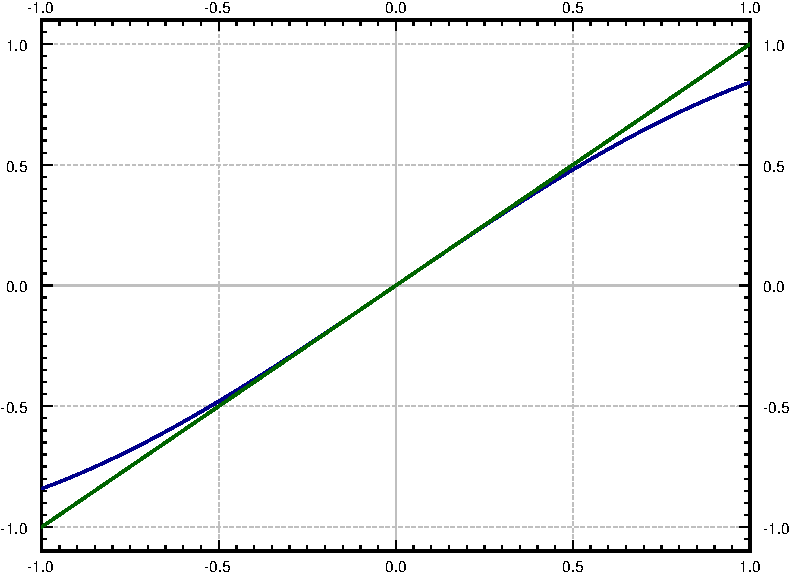
\includegraphics[width=1.5in]{../figures/mv-sintheta.pdf}

\vspace*{-0.8in}
\pause

So as long as $\theta$ is small we have roughly:

\medskip

\qquad
$
\displaystyle
\theta'' + \frac{g}{L} \theta = 0 .
$

\vspace*{12pt}

\end{frame}

\begin{frame}
We consider free motion, $F \equiv 0$.
\pause
We start with free undamped motion, $c = 0$:
\[
mx'' + kx = 0 .
\]
\pause
Let $\omega_0 = \sqrt{\nicefrac{k}{m}}$ and write
\[
x'' + \omega_0^2 x = 0 .
\]
\pause
The general solution is the \emph{simple harmonic motion}:
\[
x(t) = A \cos (\omega_0 t) + B \sin (\omega_0 t) 
\pause
\qquad
\text{or}
\qquad
x(t) = C \cos (\omega_0 t - \gamma) 
\]
\pause
First form easier to solve for initial conditions, second form
natural.

\medskip
\pause

$\omega_0$ is the (natural) \emph{angular frequency} (radians per time).

\pause
$C = \sqrt{A^2+B^2}$ is the \emph{amplitude}.

\pause
$\gamma$ is the \emph{phase shift}.

\medskip
\pause

Note:
\emph{frequency} (cycles per unit time) is
angular frequency over $2\pi$ (radians per cycle):
$\dfrac{\omega_0}{2\pi}$.

\pause

Note:
\emph{period} is the reciprocal of \emph{frequency} (time of one cycle):
$\dfrac{2\pi}{\omega_0}$.
\end{frame}

\begin{frame}
\textbf{Example:}
Suppose
$m=\unit[2]{kg}$ and $k=\unitfrac[8]{N}{m}$.

\pause
The setup sits on a truck travelling at \unitfrac[1]{m}{s}.

\pause
The truck crashes and suddenly stops.

\pause
The mass was 0.5 meters forward from the rest position and got loose during the
crash and is now moving forward at \unitfrac[1]{m}{s}.

\medskip
\pause

What is the frequency of the oscillation? \pause

What is the amplitude?

\medskip
\pause

The problem is

$2 x'' + 8 x = 0 , \quad x(0) = 0.5, \quad x'(0) = 1.$

\pause
\medskip

Angular frequency $\omega_0 = \sqrt{\nicefrac{k}{m}} = \sqrt{4} = 2$.

\medskip
\pause

Frequency in Hertz: $\nicefrac{2}{2\pi} = \nicefrac{1}{\pi} \approx 0.318$.

\medskip
\pause

The general solution is: $x(t) = A \cos (2t) + B \sin (2t)$.

\pause
$x(0) = 0.5$ \wthus $A = 0.5$.

$x'(t) = - 2(0.5) \sin (2t) + 2B \cos (2t)$.
\quad $x'(0) = 1$ \wthus $B = 0.5$.

\medskip
\pause

The amplitude is $C = \sqrt{A^2+B^2} = \sqrt{0.25+0.25} = \sqrt{0.5} \approx 0.707$
meters.

\medskip
\pause

Solution is: \quad
$x(t) = 0.5 \cos (2t) + 0.5 \sin (2t)$

\vspace*{-2.35in}%
\hspace*{3.2in}%
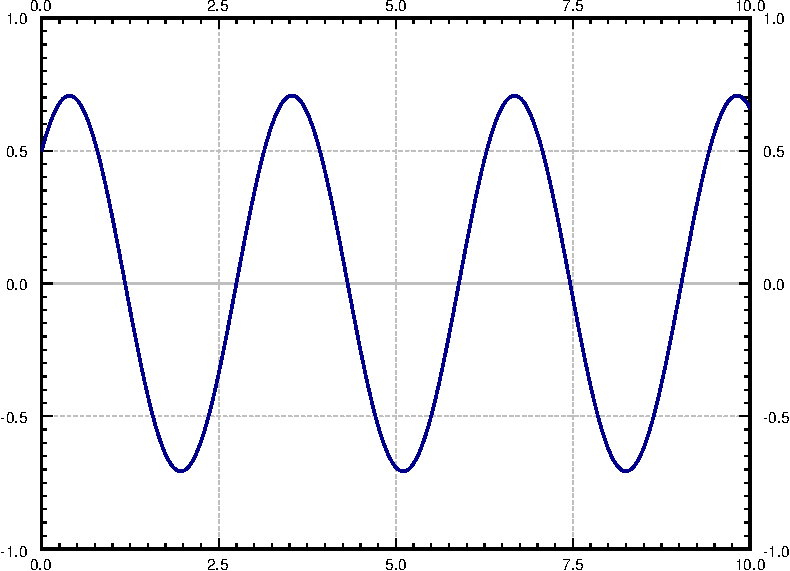
\includegraphics[width=2.3in]{../figures/mv-undamped.pdf}

\vspace*{48pt}

\end{frame}

\begin{frame}
For free undamped motion, solution is
\begin{equation*}
x(t) = A \cos (\omega_0 t) + B \sin (\omega_0 t) ,
\end{equation*}
where $x(0) = A$ and $x'(0) = \omega_0 B$.

\medskip
\pause

Amplitude $C = \sqrt{A^2+B^2}$.

\medskip
\pause

$\gamma$ is a bit harder: $\tan \gamma = \nicefrac{B}{A}$, 

\pause

One takes the arctangent but that could be $\pi$ off.

\medskip
\pause

In the example $\tan \gamma = 1$.  \quad $\arctan 1 = \nicefrac{\pi}{4}$.

\medskip
\pause

Is $\gamma = \nicefrac{\pi}{4}$? \pause  Check signs: Both $A$ and $B$ were
positive so, $(A,B)$ is in the first quadrant, no need to add $\pi$.
\pause
$\gamma = \nicefrac{\pi}{4}$.

\medskip
\pause

Basically, if $A > 0$, don't add $\pi$, if $A < 0$, then add or subtract
$\pi$. \pause
If $A = 0$, then if $B > 0$, $\gamma = \nicefrac{\pi}{2}$, if
$B < 0$, then $\gamma =\nicefrac{-\pi}{2}$.

\medskip
\pause

Calculators and computer software often have a function like
\texttt{atan2(A,B)} that computes $\gamma$.

\end{frame}

\end{document}
